\section{Implementation}
\labelsec{Implementation}
\subsection{Radar}
The console part of the radar is implemented as a web page, which is automatically generated in the \lstinline[columns=fixed, style=java]{srcMore} directory in a package associated with each Context when the \textbf{-httpserver} flag for a Context is set. It is implemented by a HTTP web-socket server working on port 8080. This interface emits different kind of events. For example, the Start button emits the event  \lstinline[columns=fixed, style=java]{cmd : cmd(start)}.
\begin{figure}[h]
	\centering
	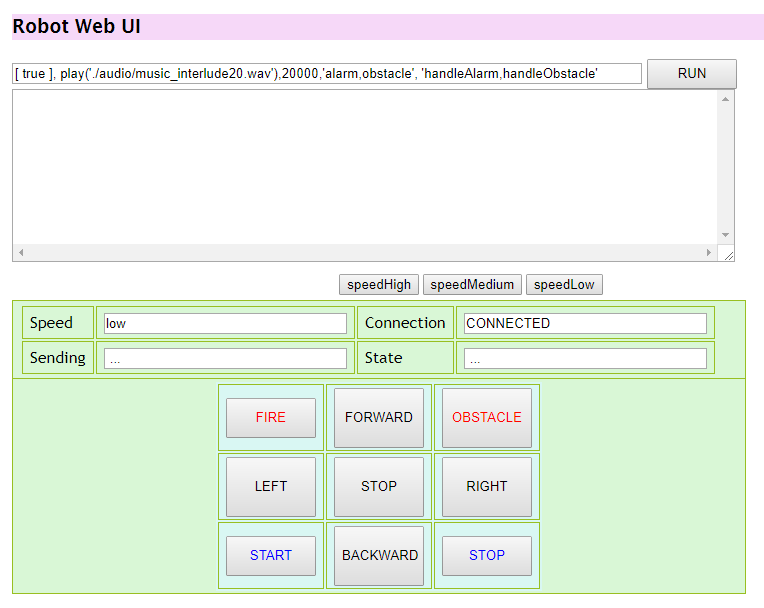
\includegraphics[width=\linewidth]{webconsole.png}
	\caption{Web console.}
\end{figure}
\\
The GUI part of the radar (where the sonars data are shown) is implemented using specific libraries provided by the software house.
\subsection{Led blinking}
The blink of the led has to be asynchronous, so that while the led is blinking, the robot can continue its operations without being blocked. In order to do so, the led is implemented as a \lstinline[columns=fixed, style=java]{SituatedActiveObject} supplied by the software house.
\lstinputlisting[style=java]{list/BlinkAsynch.java}
\subsection{Transmission of images through MQTT}
For the photo shoot through the camera, we used an open source library found on Github, called \textbf{JRPiCam} which wraps the commands needed to take a photo. Once the photo is acquired, it is converted in a String encoded with \textbf{Base64} encoding and then published on the \textbf{MQTT} broker, with a specified topic. The radar running on PC will have to decode the String received through MQTT in order to rebuild the image and then save it locally.
\lstinputlisting[style=java]{list/Camera.java}
\lstinputlisting[style=java]{list/Photoreceiver.java}
All the sonars, either on the path or on the robot, retreive the distances executing a C program called \lstinline[columns=fixed, style=java]{SonarAlone}, provided by the sofware house.
\lstinputlisting[style=java]{list/Sensorsonar.java}
The software house has already studied, in previous works, how to handle a robot-related device that by its nature can not send messages / events. When you say that an actor is a Robot, the code generator produces two files in the package reserved for the actor: a prolog theory \lstinline[columns=fixed, style=java]{sensorTheory} and a java file called \lstinline[columns=fixed, style=java]{SensorObserver}. The observer was automatically created and registered with all the sensors supplied to the robot so that they can perceive state changes: it is a task of the application designer to specify the behaviour after receiving a sensory data. To do so, you need to modify the generated prolog theory or specify the behaviour in the java file. \\
Despite this, we decided to handle the sonar on the robot the same way we handle the sonars on the path, as the data returned are far more accurate.